\chapter{Risk, Sustainability and Operations}
\section{Technical Risk Assessment}
\subsection{Likelihood \& Severity}
\label{sec: likelihood and severity}
Two metrics used to assess risk will be derived from likelihood of the risk occurring and severity of its occurrence. This is in line with standard aerospace practice and will use a \textbf{1-5} denotation for both likelihood and severity. \medskip


\noindent The likelihood table presents the probability of occurrence on a five-level scale. It follows the ECSS risk-management approach, but the probability ranges are tailored to the given mission. The adopted levels are minimum ($<$1\%), Low (1-20\%), Medium (20-50\%), High (50-80\%), and Maximum ($>$80\%), providing a project-specific but structured basis for risk scoring~\cite{ECSS_M_ST_80C_2008}.




\begin{table}[H]
\centering
\footnotesize
\renewcommand{\arraystretch}{1.3}
\setlength{\tabcolsep}{8pt}
\begin{tabular}{c l c p{8cm}}
\rowcolor{gray!20}
\textbf{Score} & \textbf{ECSS Label} & \textbf{Probability} & \textbf{Definition} \\

\rowcolor{green!20}
1 & Minimum & $<1\%$ & Would require extraordinary coincidence of failures. \\

\rowcolor{lime!30}
2 & Low & $1{-}20\%$ & Has happened occasionally in comparable design projects; needs a specific combination of factors. \\

\rowcolor{yellow!30}
3 & Medium & $20{-}50\%$ & Could happen; the team is in a territory where things have gone wrong before. \\

\rowcolor{orange!40}
4 & High & $50{-}80\%$ & More likely to occur than not; the conditions driving the risk are already partly present. \\

\rowcolor{red!40}
5 & Maximum & $>80\%$ & Expected to occur if no action is taken; the event is already partially unfolding. \\

\end{tabular}
\caption{Probability scale for organisational risk assessment}
\end{table}


\vspace*{-0.4cm}
\noindent The severity table \ref{tab:severity} defines consequences in terms of project impact, measured through effects on deliverable quality, team performance, and schedule. 



\begin{table}[H]
\centering
\footnotesize
\renewcommand{\arraystretch}{1.3}
\setlength{\tabcolsep}{8pt}
\begin{tabular}{c l p{8.5cm}}
\rowcolor{gray!20}
\textbf{Score} & \textbf{ECSS Label} & \textbf{Technical impact / scope} \\

\rowcolor{green!20}
1 & Negligible & Minor technical issue with no effect on subsystem performance \\

\rowcolor{lime!30}
2 & Moderate & Limited reduction in subsystem performance, requiring small design adjustments \\

\rowcolor{yellow!30}
3 & Significant & Noticeable degradation of subsystem performance, requiring redesign of part of the subsystem \\

\rowcolor{orange!40}
4 & Critical & Major subsystem performance loss, requiring substantial redesign or replacement of key components \\

\rowcolor{red!40}
5 & Catastrophic & Failure of the subsystem to meet its main function, threatening mission feasibility \\

\end{tabular}
\caption{Severity scale for technical risk assessment}
\label{tab:severity}
\end{table}

\subsection{Risks Table}
\label{sec:riskstable}

The scale ranges from negligible, where the impact is absorbed within the same day, to catastrophic, where the impact threatens the project deadline or final review. This follows the ECSS risk-management approach of treating severity separately from likelihood, while adapting the consequence definitions to the 10-week DSE context\cite{ECSS_M_ST_80C_2008}. This table lists all the risks that have been identified so far and their respective contingency measures. They have been categorised into seven subgroups, which can be identified by the middle letters in the risk ID. Also, as explained previously, pre- and post-mitigation probability and severity have been assigned to each risk, and are denoted by $P_b$, $S_b$, $P_a$, $S_a$, respectively. Finally, a person who is responsible for that specific risk mitigation has been identified.

\begin{spacing}{0.95}
\begingroup
\scriptsize
\setlength{\tabcolsep}{2pt}
\renewcommand{\arraystretch}{1.18}

\begin{longtable}{@{}
>{\raggedright\arraybackslash}p{0.08\textwidth}
>{\raggedright\arraybackslash}p{0.18\textwidth}
>{\raggedright\arraybackslash}p{0.27\textwidth}
>{\centering\arraybackslash}p{0.035\textwidth}
>{\centering\arraybackslash}p{0.035\textwidth}
>{\centering\arraybackslash}p{0.04\textwidth}
>{\centering\arraybackslash}p{0.035\textwidth}
>{\centering\arraybackslash}p{0.035\textwidth}
>{\centering\arraybackslash}p{0.04\textwidth}
>{\raggedright\arraybackslash}p{0.12\textwidth}
@{}}

\caption{Technical Risk Assessment and Mitigation Overview, where $R_b=P_bS_b$ and $R_a=P_aS_a$}
\label{tab:technical_risk_assessment} \\

\toprule
\textbf{Risk ID} &
\textbf{Risk} &
\textbf{Contingency or Prevention} &
\textbf{$P_b$} &
\textbf{$S_b$} &
\textbf{$R_b$} &
\textbf{$P_a$} &
\textbf{$S_a$} &
\textbf{$R_a$} &
\textbf{Responsible Person} \\
\midrule
\endfirsthead

\toprule
\textbf{Risk ID} &
\textbf{Risk} &
\textbf{Contingency or Prevention} &
\textbf{$P_b$} &
\textbf{$S_b$} &
\textbf{$R_b$} &
\textbf{$P_a$} &
\textbf{$S_a$} &
\textbf{$R_a$} &
\textbf{Responsible Person} \\
\midrule
\endhead

\midrule
\multicolumn{10}{r}{\small Continued on next page} \\
\endfoot

\bottomrule
\endlastfoot

\multicolumn{10}{@{}l}{\textbf{Manufacturing}} \\
\midrule

TR-MA-01 & Delays in the manufacturing process &
Have a backup manufacturer ready, or account for potential delays in Gantt chart. &
4 & 3 & \textbf{12} & 2 & 2 & \textbf{4} & Structures Engineer \\

TR-MA-02 & Damage during the folding and packaging of the balloon &
Use controlled handling procedures, secure packaging, and careful assessment before final assembly. &
1 & 5 & \textbf{5} & 1 & 4 & \textbf{4} & Structures Engineer / Systems Engineer \\

TR-MA-03 & Late identification of defects may delay the launch &
Schedule testing procedures while accounting for possible repair procedures, and keep spare components for critical subsystems. &
2 & 3 & \textbf{6} & 1 & 2 & \textbf{2} & Structures Engineer / Systems Engineer \\

TR-MA-04 & Integration mismatch between balloon, gondola, inflation system, and parachute may cause deployment issues &
Conduct full-scale checks to ensure all systems function well together. Rehearse the deployment before final assembly if possible. &
1 & 4 & \textbf{4} & 1 & 3 & \textbf{3} & Systems Engineer \\

TR-MA-05 & Immature or unreliable manufacturing methods may prevent the required techno- logy from achieving required TRL before launch &
Ensure a backup is available, such as older technology that is still reliable, in case qualification tests fail. &
2 & 3 & \textbf{6} & 2 & 2 & \textbf{4} & Systems Engineer \\

TR-MA-06 & Mass growth during manufacturing may exceed the allocated mass budget &
Keep track of mass continuously and include a mass margin for late manufacturing changes. &
3 & 3 & \textbf{9} & 2 & 2 & \textbf{4} & Cost \& Budget Controller \\

\multicolumn{10}{@{}l}{\textbf{Launch}} \\
\midrule

TR-LAU-01 & Launch delay &
Plan according to weather expectations during certain seasons, keep the S/C in a safe storage location, keep the trajectory for the next launch window updated, and prepare backup launch data. &
4 & 1 & \textbf{4} & 3 & 1 & \textbf{3} & Systems Engineer \\

TR-LAU-02 & S/C incapable of handling launch loads &
Verify structural margins before launch through analysis and load testing. In case of failure during launch, place the spacecraft in a safe configuration to prevent further damage while diagnosing which systems should not be turned on. &
2 & 5 & \textbf{10} & 1 & 4 & \textbf{4} & Structures Engineer \\

TR-LAU-03 & S/C incapable of handling launch vibrations &
Verify structural margins before launch through analysis and vibration testing. In case of failure during launch, place the spacecraft in a safe configuration to prevent further damage while diagnosing which systems should not be turned on. &
2 & 5 & \textbf{10} & 1 & 4 & \textbf{4} & Structures Engineer \\

TR-LAU-04 & S/C damaged by pyroshock during separation &
Use shock qualification testing and shock isolators. After separation, perform health checks, switch to backup units if needed, and place the spacecraft in a safe configuration while diagnosing damage. &
1 & 5 & \textbf{5} & 1 & 4 & \textbf{4} & Structures Engineer \\

TR-LAU-05 & S/C damaged by pressure or thermal changes during ascent &
Design the spacecraft for the expected ascent environment, use thermal protection and venting paths, check pressure-sensitive components and electronics after launch, and switch to redundant systems if degradation is detected. &
1 & 5 & \textbf{5} & 1 & 5 & \textbf{5} & Structures Engineer \\

TR-LAU-06 & Launcher explodes or fails during ascent &
Use mission insurance and replacement spacecraft planning to rebuild the spacecraft. &
1 & 5 & \textbf{5} & 1 & 4 & \textbf{4} & Systems Engineer \\

TR-LAU-07 & Stage separation failure &
Use redundant separation mechanisms, backup separation commands, and technical verification before launch. &
2 & 5 & \textbf{10} & 1 & 4 & \textbf{4} & Systems Engineer \\

TR-LAU-08 & Damage from debris in Earth orbit &
Track debris before and after launch, adjust parking orbit or timing if needed, and use shielding for critical components. &
1 & 4 & \textbf{4} & 1 & 3 & \textbf{3} & Structures Engineer \\

TR-LAU-09 & Launcher fails to insert S/C into Earth orbit &
Use onboard propulsion to correct the orbit if the error is small, keep propellant margin for emergency correction, and prepare a backup mission profile if the nominal Venus transfer is no longer possible. &
2 & 5 & \textbf{10} & 1 & 4 & \textbf{4} & Systems Engineer \\

TR-LAU-10 & Launcher puts S/C in wrong transfer orbit &
Recalculate the orbit manoeuvre required for Venus orbit immediately, or prepare probable failure trajectories beforehand. Use onboard propulsion and backup fuel to correct the orbit. &
2 & 5 & \textbf{10} & 2 & 4 & \textbf{8} & Systems Engineer \\

TR-LAU-11 & Venus orbit insertion fails &
Attempt a backup burn using the main engine or smaller thrusters. &
2 & 5 & \textbf{10} & 1 & 4 & \textbf{4} & Systems Engineer \\

TR-LAU-12 & Fairing separation failure &
Use redundant fairing separation systems and attempt backup separation commands if the first command fails. &
1 & 5 & \textbf{5} & 1 & 5 & \textbf{5} & Mechanisms Engineer \\

TR-LAU-13 & Spacecraft separation failure &
Attempt redundant separation commands, backup pyrotechnic devices, or spring-release systems. &
2 & 5 & \textbf{10} & 2 & 5 & \textbf{10} & Mechanisms Engineer \\

\multicolumn{10}{@{}l}{\textbf{Deployment}} \\
\midrule

TR-D-01 & Parachute failure during deployment &
Conduct deployment testing before launch, use a reliable parachute design, and ensure that there is a backup parachute. &
2 & 5 & \textbf{10} & 1 & 2 & \textbf{2} & Deployment Engineer \\

TR-D-02 & Balloon inflation failure &
Ensure alternative inflation paths and pressure monitoring. Include enough inflation margin to complete deployment. &
1 & 5 & \textbf{5} & 1 & 3 & \textbf{3} & Deployment Engineer \\

TR-D-03 & Incorrect deployment sequence or timing &
Test the deployment sequence in advance with correct deployment logic and sufficient timing margins. &
2 & 5 & \textbf{10} & 1 & 5 & \textbf{5} & Deployment Engineer \\

TR-D-04 & Gondola instability after deployment &
Simulate the descent a sufficient number of times, including damping, proper mass distribution, and stability. &
3 & 5 & \textbf{15} & 2 & 4 & \textbf{8} & Deployment Engineer \\

TR-D-05 & Communication loss during deployment &
Use an autonomous deployment sequence and store deployment telemetry onboard. &
3 & 3 & \textbf{9} & 2 & 2 & \textbf{4} & Deployment Engineer \\

TR-D-06 & Loss of control during Re-entry &
Design for stability and resistance to tumbling, verify stability through CFD and re-entry simulations, include attitude-control/passive-stability margins &
1 & 5 & \textbf{5} & 1 & 5 & \textbf{5} & Deployment Engineer \\

\multicolumn{10}{@{}l}{\textbf{Payload}} \\
\midrule

TR-PL-01 & Aerosampling system fails &
Use redundant sampling paths, add particle filters or mesh screens to prevent clogging by cloud aerosols, and include a self-cleaning cycle. &
2 & 4 & \textbf{8} & 1 & 3 & \textbf{3} & Payload Engineer \\

TR-PL-02 & Certain or all measurement devices cannot handle the Venus environment &
Select sensors with proper thermal, pressure, and chemical compatibility. Place sensitive components in a sealed and thermally controlled gondola compartment, use external sensors only where needed, and add sensor redundancy. &
1 & 4 & \textbf{4} & 1 & 4 & \textbf{4} & Payload Engineer \\

TR-PL-03 & Chemical analysis measurement device fails or produces faulty data &
Include redundant critical components, use a simplified robust chemical-analysis system, add internal reference gases so the system can check itself, and design to avoid cross-contamination between samples. &
2 & 3 & \textbf{6} & 1 & 3 & \textbf{3} & Payload Engineer \\

TR-PL-04 & Seismic/infrared payload device cannot detect Venus-quakes clearly &
Use multiple detection methods, switch to safe diagnostic mode, and attempt recovery using backup sensors, recalibration, or updated ground-based data-processing filters. If recovery is not possible, continue with reduced science operations using atmospheric data. &
3 & 4 & \textbf{12} & 2 & 3 & \textbf{6} & Payload Engineer \\

\multicolumn{10}{@{}l}{\textbf{Other Subsystems}} \\
\midrule

TR-OS-01 & On-board computer failure &
Include fault detection and timed automatic reboot. &
1 & 5 & \textbf{5} & 1 & 3 & \textbf{3} & Comms \& Data Engineer \\

TR-OS-02 & Data handling memory failure may result in loss of scientific data &
Ensure there is a backup so that important data is duplicated and safely stored. &
2 & 4 & \textbf{8} & 2 & 2 & \textbf{4} & Comms \& Data Engineer \\

TR-OS-03 & The data rate constraint of 1500 bit/s is exceeded &
Compress data onboard, reduce sampling frequency during quiet periods, prioritise high-value science and health data, store excess data locally, and coordinate with payload and data-handling teams to reduce generated data. &
3 & 1 & \textbf{3} & 1 & 1 & \textbf{1} & Comms \& Data Engineer \\

TR-OS-04 & The energy storage needed exceeds 500 Wh &
Negotiate the constraint, coordinate with all subsystem departments to reduce energy storage needs, and re-evaluate the mission schedule to separate high-energy tasks. &
3 & 2 & \textbf{6} & 1 & 2 & \textbf{2} & EPS Engineer \\

TR-OS-05 & Fatigue structural failure due to long mission time &
Perform testing beforehand and analyse known fatigue data of the involved elements. In case of in-flight structural failure, change altitude to reduce loads on the aerobot. &
3 & 4 & \textbf{12} & 2 & 2 & \textbf{4} & Structures Engineer \\

TR-OS-06 & Thermal control system fails &
Use insulation, coatings, heaters/coolers, and Venus-environment testing before launch. In flight, switch off non-essential payloads, reduce power dissipation, and change altitude to a more favourable temperature region if possible. &
2 & 3 & \textbf{6} & 2 & 2 & \textbf{4} & Thermal Engineer \\

TR-OS-07 & Power system fails &
Switch to battery safe mode, or complete shutdown of all non-critical subsystems except essential command-execution systems while the ground team attempts to solve the power-system issue. &
2 & 5 & \textbf{10} & 2 & 4 & \textbf{8} & EPS Engineer \\
TR-OS-08 & Communication subsystem degradation prevents regular data downlink &
Include low-rate emergency telemetry, redundant communication paths where possible, onboard data buffering, and prioritisation of critical housekeeping data until contact is restored. &
2 & 5 & \textbf{10} & 1 & 4 & \textbf{4} & Comms \& Data Engineer \\

TR-OS-09 & Antenna, RF cable, or connector degradation reduces link margin &
Use environmental qualification, RF continuity checks, conservative link margin, robust cable routing, and two-antenna placement to reduce blockage and single-point RF failures. &
2 & 4 & \textbf{8} & 1 & 3 & \textbf{3} & Comms \& Data Engineer \\

TR-OS-10 & ISRU/buoyancy-control valve or pump failure prevents altitude regulation &
Use pressure monitoring, redundant or fail-safe valves, conservative buoyancy margins, and autonomous fallback modes that minimise power use while maintaining science or survival operation. &
2 & 5 & \textbf{10} & 1 & 4 & \textbf{4} & ISRU / Buoyancy Engineer \\

TR-OS-11 & IMU or navigation-sensor failure degrades motion correction and altitude-state estimation &
Cross-check IMU data with barometers and housekeeping sensors, flag affected science data, switch to pressure-based altitude estimation, and continue reduced-accuracy science operations. &
2 & 3 & \textbf{6} & 1 & 2 & \textbf{2} & Comms \& Data Engineer / Payload Engineer \\

TR-OS-12 & Subsystem interface bus failure prevents command or telemetry exchange with one or more units &
Use interface timeout detection, isolate the failed bus or node, route around failed devices where possible, and place affected subsystems in a predefined safe configuration. &
2 & 4 & \textbf{8} & 1 & 3 & \textbf{3} & Comms \& Data Engineer \\
\multicolumn{10}{@{}l}{\textbf{Budget}} \\
\midrule

TR-B-01 & Total expected mission budget exceeds \EUR 400 million &
Descope the mission by reducing non-essential payload functions, simplifying the aerobot design, using fewer redundant components where acceptable, and focusing on core-science objectives. &
3 & 4 & \textbf{12} & 2 & 3 & \textbf{6} & Cost \& Budget Controller \\

TR-B-02 & Mission must survive 5 years, so operations cost could grow too high due to certain events &
Use less frequent ground contact, more autonomous onboard operations, and incorporate expected higher operations cost in the budget. &
3 & 3 & \textbf{9} & 2 & 2 & \textbf{4} & Cost \& Budget Controller \\

\multicolumn{10}{@{}l}{\textbf{Environment}} \\
\midrule

TR-ENV-01 & The aerobot ends up above the habitable zone &
Make sure the altitude control devices work as intended, such that when the balloon rises above the intended altitude, it is returned quickly &
1 & 3 & \textbf{3} & 1 & 1 & \textbf{1} & Deployment \\

TR-ENV-02 & The aerobot ends up in the pole vortices &
In case this happens, turn off non-critical systems to save power and obtain valuable in-situ data from poles till the end-of-lifetime &
1 & 5 & \textbf{5} & 1 & 4 & \textbf{4} & Deployment \\

TR-ENV-03 & Aerobot surface degrades due to prolonged exposure to Venus' sulfuric-acid cloud droplets &
Use acid-resistant fluoropolymer/metalised barrier coatings and sacrificial outer layers &
4 & 3 & \textbf{12} & 3 & 2 & \textbf{6} & Materials \\

\end{longtable}

\endgroup

\end{spacing}

\noindent Risk identification is carried out by constructing a risk matrix that compares the likelihood and severity of different risk scenarios. This provides a clear overview of the overall importance of each scenario. 

\noindent The coloured regions indicate the priority of preventive action: green risks are acceptable and require only monitoring, yellow risks call for active mitigation, and red risks are unacceptable and require immediate response. For example, a moderate severity event of rare likelihood may fall within the green region, whereas a major severity event with a likely chance is classified as red. The Pre-mitigation risk map in \autoref{tab:premitimap} shows risk distribution before any preventive measures are applied.


\begin{table}[H]
\centering
\caption{Pre-mitigation risk map}
\scriptsize
\renewcommand{\arraystretch}{1.4}
\setlength{\tabcolsep}{3pt}

\begin{tabular}{>{\raggedright\arraybackslash}p{3.6cm}|
>{\centering\arraybackslash}p{2.1cm}|
>{\centering\arraybackslash}p{2.1cm}|
>{\centering\arraybackslash}p{2.1cm}|
>{\centering\arraybackslash}p{2.1cm}|
>{\centering\arraybackslash}p{2.4cm}}
\rowcolor{gray!20}
\textbf{Likelihood $\downarrow$ / Severity $\rightarrow$} 
& \textbf{1} & \textbf{2} & \textbf{3} & \textbf{4} & \textbf{5} \\

\rowcolor{gray!10}
& \textbf{Negligible} 
& \textbf{Moderate} 
& \textbf{Significant} 
& \textbf{Critical} 
& \textbf{Catastrophic} \\

\textbf{A — Minimum}
& \cellcolor{green!20} 
& \cellcolor{green!20} 
& \cellcolor{green!20} TR-ENV-01
& \cellcolor{yellow!30} TR-MA-04 \newline TR-LAU-08 \newline TR-PL-02 
& \cellcolor{yellow!30} TR-MA-02 \newline TR-LAU-04 \newline TR-LAU-05 \newline TR-LAU-06 \newline TR-LAU-12 \newline TR-D-02 \newline TR-OS-01 \newline TR-D-06 \newline TR-ENV-02 \\

\textbf{B — Low}
& \cellcolor{green!20} 
& \cellcolor{green!20} 
& \cellcolor{yellow!30} TR-MA-03 \newline TR-MA-05 \newline TR-PL-03 \newline TR-OS-06 \newline TR-OS-11
& \cellcolor{yellow!30} TR-PL-01 \newline TR-OS-02 \newline TR-OS-09 \newline TR-OS-12
& \cellcolor{yellow!30} TR-LAU-02 \newline TR-LAU-03 \newline TR-LAU-07 \newline TR-LAU-09 \newline TR-LAU-10 \newline TR-LAU-11 \newline TR-LAU-13 \newline TR-D-01 \newline TR-D-03 \newline TR-OS-07 \newline TR-OS-08 \newline TR-OS-10 \\

\textbf{C — Medium}
& \cellcolor{green!20} TR-OS-03
& \cellcolor{yellow!30} TR-OS-04
& \cellcolor{yellow!30} TR-MA-06 \newline TR-D-05 \newline TR-B-02
& \cellcolor{yellow!30} TR-PL-04 \newline TR-OS-05 \newline TR-B-01 \newline TR-ENV-03
& \cellcolor{red!30} TR-D-04 \\

\textbf{D — High}
& \cellcolor{yellow!30} TR-LAU-01
& \cellcolor{yellow!30} 
& \cellcolor{yellow!30} TR-MA-01
& \cellcolor{red!30} 
& \cellcolor{red!30} \\

\textbf{E — Maximum}
& \cellcolor{yellow!30} 
& \cellcolor{yellow!30} 
& \cellcolor{red!30} 
& \cellcolor{red!30} 
& \cellcolor{red!30} \\

\end{tabular}
\label{tab:premitimap}
\end{table}

\noindent After implementing the measures listed in the previous risk table, both the likelihood and severity of several risks are reduced. The extent of this reduction varies depending on the effectiveness of the specific mitigation measures. The resulting post-mitigation risk map is shown in \autoref{tab:postmitimap}.

\begin{table}[H]
\centering
\caption{Post-mitigation risk map}
\scriptsize
\renewcommand{\arraystretch}{1.4}
\setlength{\tabcolsep}{3pt}

\begin{tabular}{>{\raggedright\arraybackslash}p{3.6cm}|
>{\centering\arraybackslash}p{2.1cm}|
>{\centering\arraybackslash}p{2.1cm}|
>{\centering\arraybackslash}p{2.1cm}|
>{\centering\arraybackslash}p{2.1cm}|
>{\centering\arraybackslash}p{2.4cm}}
\rowcolor{gray!20}
\textbf{Likelihood $\downarrow$ / Severity $\rightarrow$} 
& \textbf{1} & \textbf{2} & \textbf{3} & \textbf{4} & \textbf{5} \\

\rowcolor{gray!10}
& \textbf{Negligible} 
& \textbf{Moderate} 
& \textbf{Significant} 
& \textbf{Critical} 
& \textbf{Catastrophic} \\

\textbf{A — Minimum}
& \cellcolor{green!20} TR-OS-03 \newline TR-ENV-01
& \cellcolor{green!20} TR-MA-03 \newline TR-D-01 \newline TR-OS-04 \newline TR-OS-11
& \cellcolor{green!20} TR-MA-04 \newline TR-LAU-08 \newline TR-D-02 \newline TR-PL-01 \newline TR-PL-03 \newline TR-OS-01 \newline TR-OS-09 \newline TR-OS-12
& \cellcolor{yellow!30} TR-MA-02 \newline TR-LAU-02 \newline TR-LAU-03 \newline TR-LAU-04 \newline TR-LAU-06 \newline TR-LAU-07 \newline TR-LAU-09 \newline TR-LAU-11 \newline TR-PL-02 \newline TR-ENV-02 \newline TR-OS-08 \newline TR-OS-10
& \cellcolor{yellow!30} TR-LAU-05 \newline TR-LAU-12 \newline TR-D-03 \newline TR-D-06 \\

\textbf{B — Low}
& \cellcolor{green!20} 
& \cellcolor{green!20} TR-MA-01 \newline TR-MA-05 \newline TR-MA-06 \newline TR-D-05 \newline TR-OS-02 \newline TR-OS-05 \newline TR-OS-06 \newline TR-B-02
& \cellcolor{yellow!30} TR-PL-04 \newline TR-B-01
& \cellcolor{yellow!30} TR-LAU-10 \newline TR-D-04 \newline TR-OS-07
& \cellcolor{yellow!30} TR-LAU-13 \\

\textbf{C — Medium}
& \cellcolor{green!20} TR-LAU-01
& \cellcolor{yellow!30} TR-ENV-03
& \cellcolor{yellow!30} 
& \cellcolor{yellow!30} 
& \cellcolor{red!30} \\

\textbf{D — High}
& \cellcolor{yellow!30} 
& \cellcolor{yellow!30} 
& \cellcolor{yellow!30} 
& \cellcolor{red!30} 
& \cellcolor{red!30} \\

\textbf{E — Maximum}
& \cellcolor{yellow!30} 
& \cellcolor{yellow!30} 
& \cellcolor{red!30} 
& \cellcolor{red!30} 
& \cellcolor{red!30} \\

\end{tabular}
\label{tab:postmitimap}
\end{table}


\section{Operations}
The VISTA mission operation concepts describes how the aerobot is developed, launched, deployed and operated in the atmosphere of Venus. As seen in \autoref{fig:Timeline}, the mission is divided into two main parts: Design and assembly, and Launch and Operations. The former contains three phases which all take place on Earth and include planning, tradeoffs, subsystem interfaces development and preliminary design. The latter on the other hand includes launch in late 2035, transfer to Venus, deployment and further operations until 2041, including subsequent end-of-life procedure. 
\begin{figure}[H]
    \centering
    \makebox[\textwidth][c]{%
        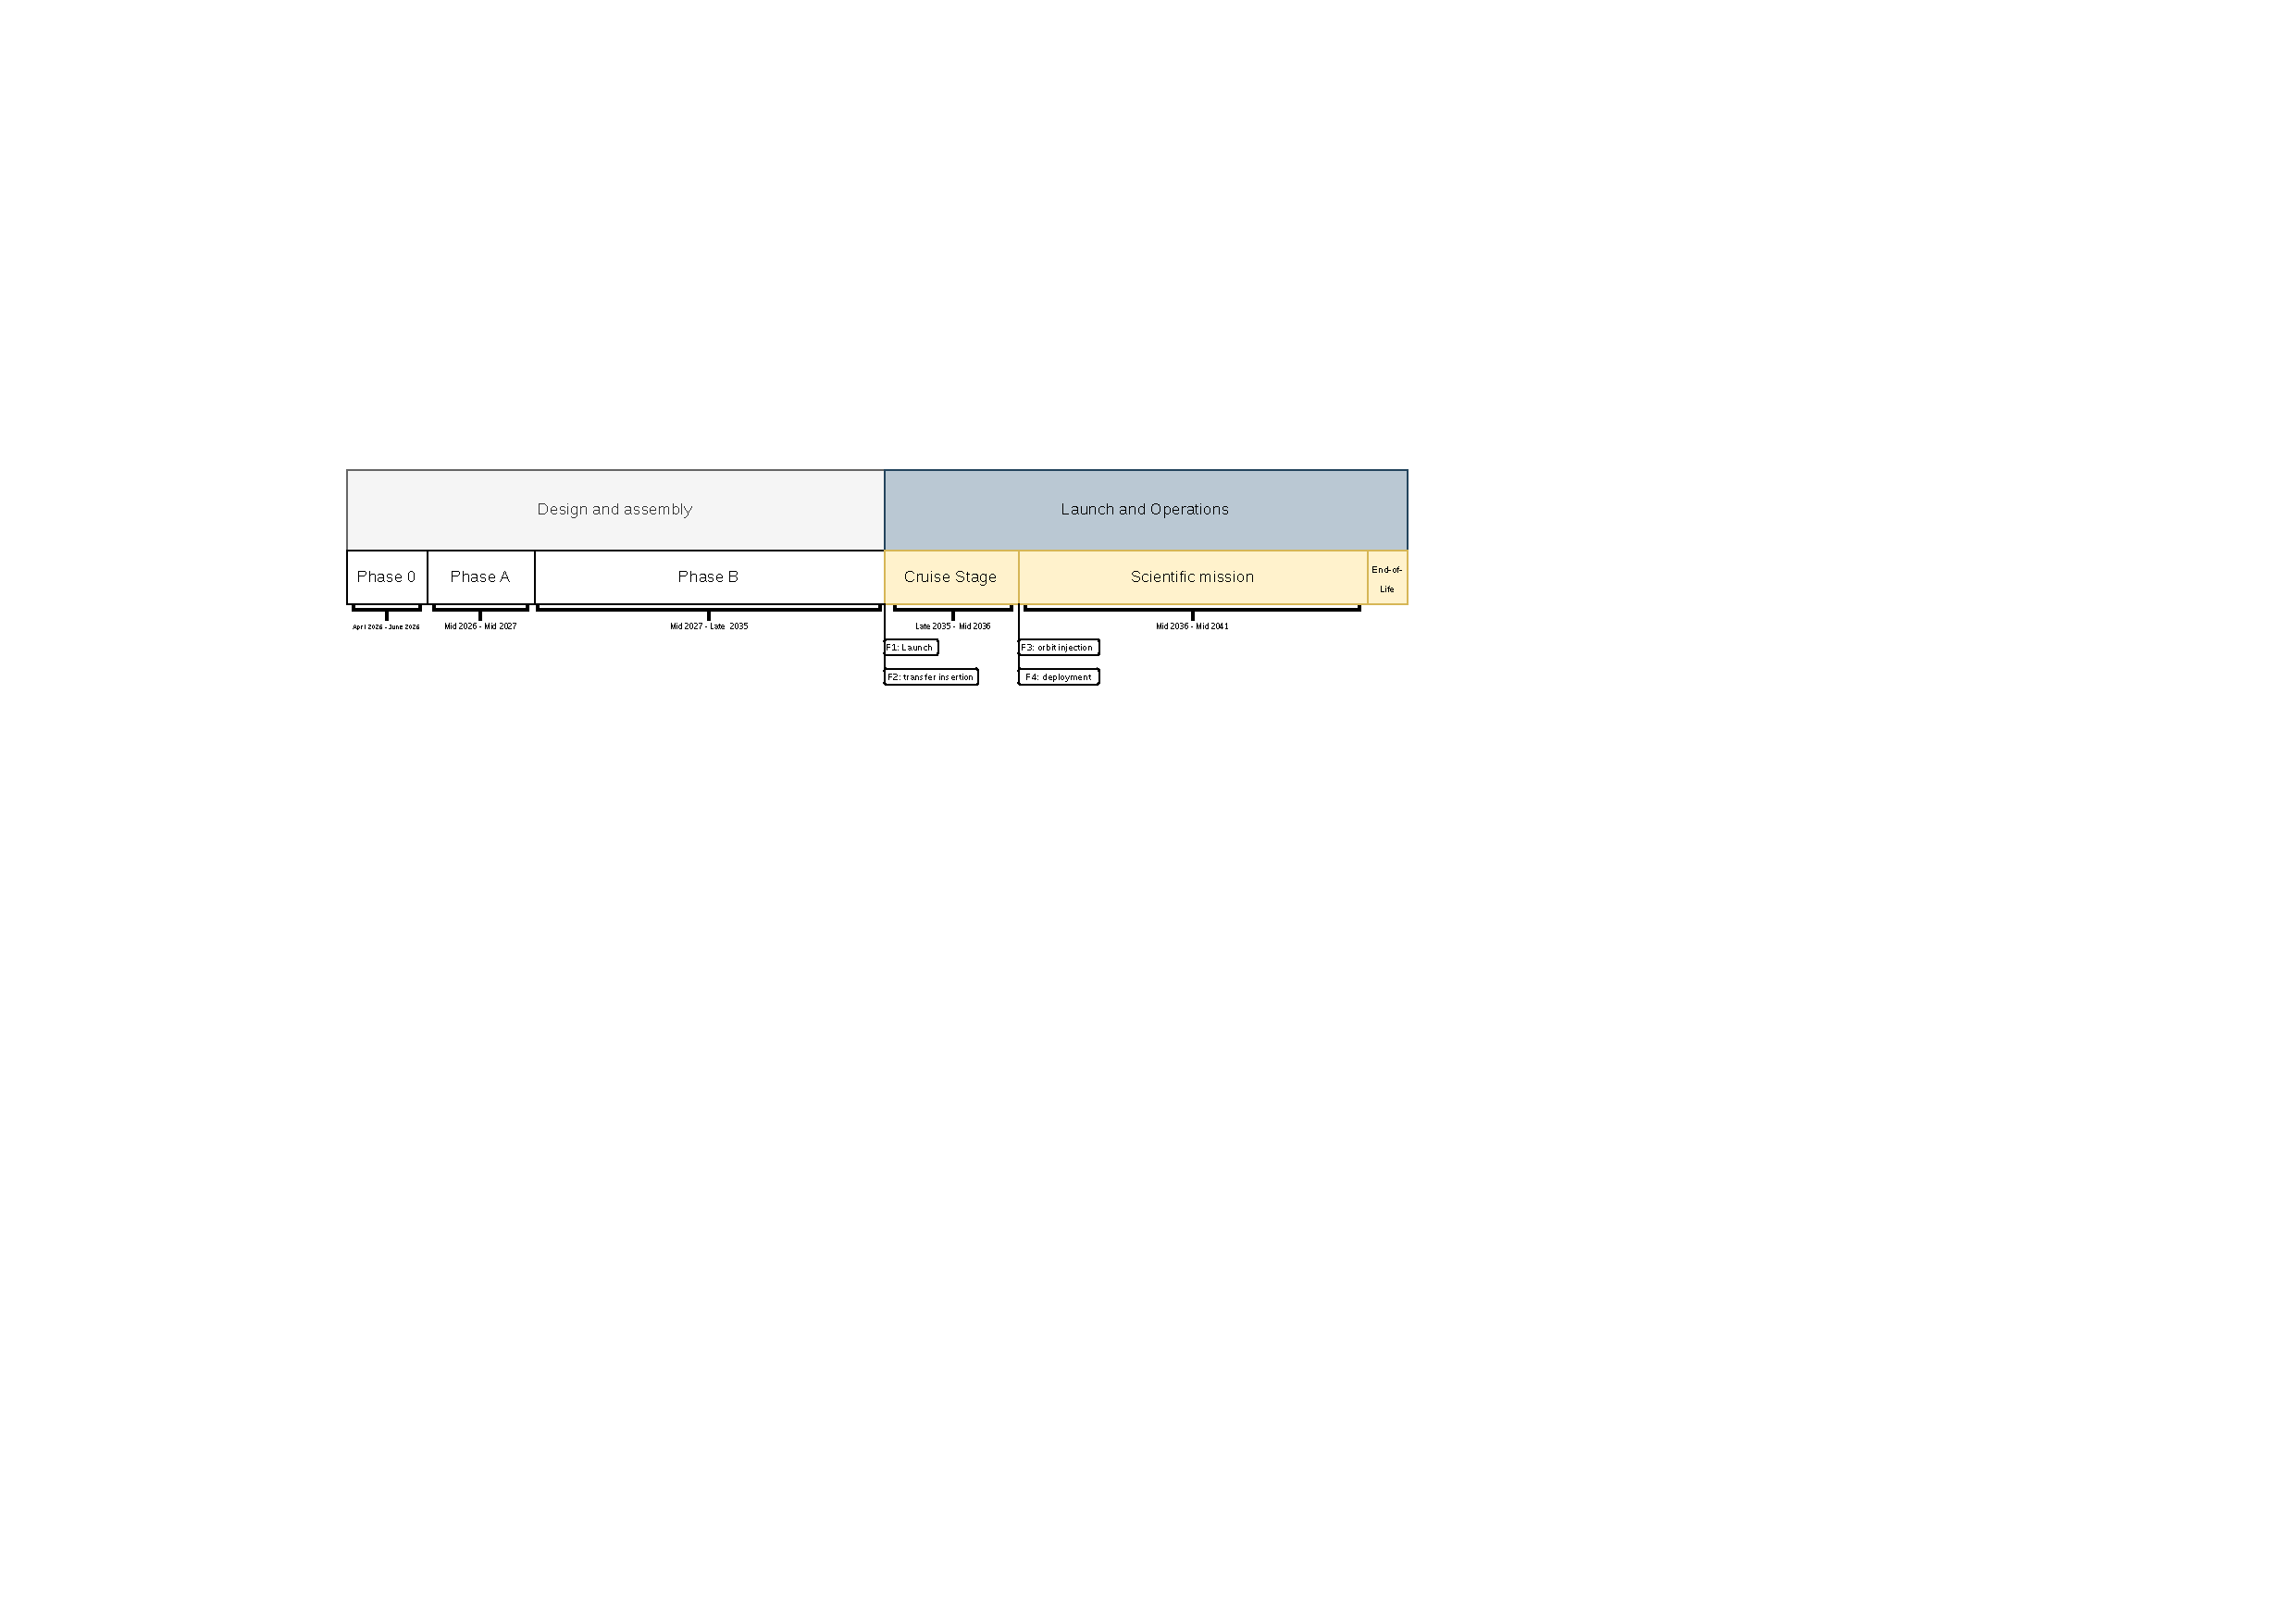
\includegraphics[width=1.2\textwidth]{fig/Operations.drawio.pdf}
    }
    \caption{Timeline}
    \label{fig:Timeline}
\end{figure}

Phase 0 sets the basic scope of the mission. For VISTA, this means defining what parts of the mission are actually designed, which include the aerobot and deployment stage, as well as verifying that the aerobot is able to perform all the required mission objectives. Other elements, such as the launcher, orbiter and ground station, are not designed in detail; however, their interfaces with VISTA are taken into consideration. Phase 0 is expected to last for the length of the DSE project.
\vspace{0.2cm}
\newline
Phase A focuses on developing the mission from an idea into a feasible concept. All mission architecture options are compared and evaluated, including the balloon architecture, in-situ resource utilization, altitude control, payload and communication strategy. The main objective of this stage is to identify a concept that is able to comply with all the requirements, while also taking into consideration and mitigating technical risks that might arise during the mission.
\vspace{0.2cm}
\newline
Phase B includes the manufacturing, assembly and testing activities, which are set to last for 8 years, until launch. At this stage, the selected VISTA concept is turned into a launch-ready system. During this stage, all subsystem layouts, mass and power budgets, the deployment sequence and verification activities are finalised. By the end of this stage, VISTA is assumed to be assembled, tested and launch-ready.






The mission operations can be seen in \autoref{fig:Con-of-op}.  
\begin{figure}[H]
    \centering
    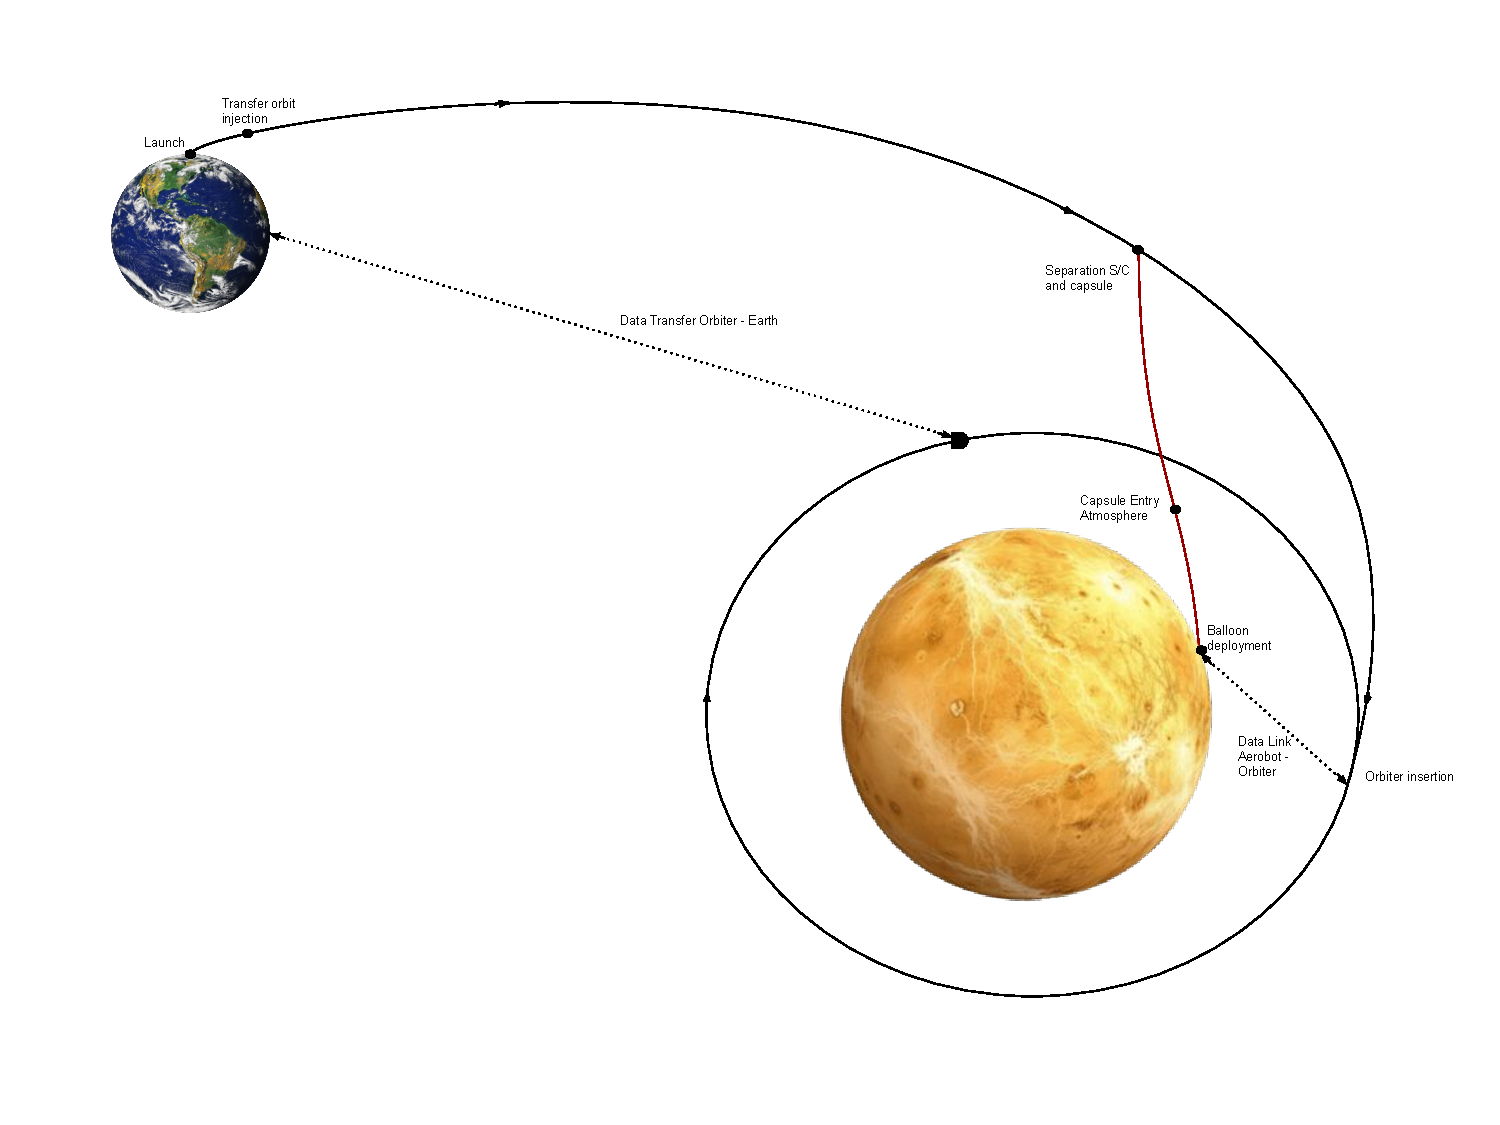
\includegraphics[width=1\linewidth]{fig/Operations.pdf}
    \caption{Concept of operation}
    \label{fig:Con-of-op}
\end{figure}
The VISTA mission follows a relay-based operational concept. After launch, the cruise stage performs the transfer to Venus while maintaining the orbiter and VISTA vehicle. Near arrival, the VISTA vehicle separates and enters the Venusian atmosphere, while the orbiter performs Venus orbit insertion. The deployment stage protects the aerobot during entry and inflation, after which the balloon-gondola system begins stable flight in the cloud layer and the deployment hardware is discarded.

During nominal operations, the aerobot performs atmospheric and seismic measurements, stores science and housekeeping data, and manages altitude through the ISRU and buoyancy subsystem. Communication relies on ESA's existing ESTRACK infrastructure, with the Venus orbiter relaying data between Mission Control and the aerobot during scheduled contact windows. At end of life, a decision is made to continue the mission or safely dispose the aerobot.






\section{Sustainability}
\label{sec:sustainability}
\todo{someone proofread pls - not too short?}

A full Life Cycle Assessment is outside the scope of the current design phase, but sustainability is considered across development, manufacturing, testing, launch, transfer, operations, and end-of-life.

The design prioritizes commercial off-the-shelf components where possible to reduce custom development effort, material waste, and manufacturing resources. Environmentally critical materials, such as high-energy batteries or acid-resistant coatings, are used only where required by the Venus environment and shall be reassessed during detailed design for lower-impact alternatives where feasible. Testing shall rely on simulations, engineering models, and combined test campaigns where possible to reduce repeated hardware production and facility use.

Since launch is expected to be a major contributor to environmental impact, spacecraft mass reduction and an efficient transfer trajectory are important mission sustainability considerations. During operations, existing and shared ground infrastructure shall be used for mission control to avoid unnecessary new facilities and reduce operational energy demand. 

At end-of-life, the aerobot is expected to remain in the Venus environment; therefore, the design shall minimize unnecessary hazardous materials, avoid avoidable contamination release, and remain compliant with applicable COSPAR planetary-protection requirements \cite{ECSS_U_ST_20C_2019} for Venus. Material choices and disposal assumptions shall be documented for future planetary-protection and end-of-life assessment.